\section{HDF5 Überblick}
\begin{frame}
	\frametitle{HDF5 (Hierarchical Data Format 5)}
			\begin{itemize}
				\item Datenmodell
					\begin{itemize}
						\item kann sehr komplexe Datenobjekte und diverse Metadaten repräsentieren
					\end{itemize}
				\item Bibliothek
					\begin{itemize}
						\item ist gleichermaßen geeignet für PCs als auch HPC
						\item implementiert C, C++, Fortran 90 und Java Schnittstellen
					\end{itemize}
				\item Dateiformat
					\begin{itemize}
						\item ist portabel und ohne Größebeschränkung
					\end{itemize}
				\item Leistungsfeatures
					\begin{itemize}
						\item für die Zugriffszeit- und Speicheroptimierungen
					\end{itemize}
				\item Tools
					\begin{itemize}
						\item zur Verwaltung, Manipulation, Darstellung und Analyse 
					\end{itemize}
			\end{itemize}

			%\begin{itemize}
				%\item selbstbeschreibend
				%\item portabel
				%\item weit verbreitet
					%\begin{itemize}
						%\item Klimaforschung, Finanzwesen, Ingenieurswissenschaften
						%%\item DKRZ, MPI, NASA
					%\end{itemize}
				%\item sehr grosse Datenmenge
					%\begin{itemize}
						%\item Klimadaten, Simulationsdaten, Sensordaten
					%\end{itemize}
			%\end{itemize}
\end{frame}

\begin{frame}
	\frametitle{Warum HDF5?}
	\begin{figure}
		\centering
		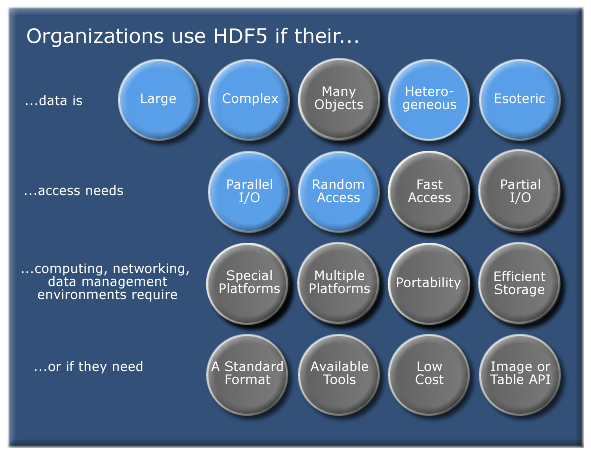
\includegraphics[width=0.8\textwidth]{pictures/why.jpg}
		\caption*{Warum HDF? [1]}
	\end{figure}
\end{frame}

%\begin{frame}
	%\frametitle{HDF5 E/A-Features}
	%\includegraphics[width=0.5\textwidth]{pictures/Dsets_fig16.JPG}
%\end{frame}end{frame}

\begin{frame}
	\frametitle{HDF5 VOL-Architektur}
	\begin{figure}
		\centering
		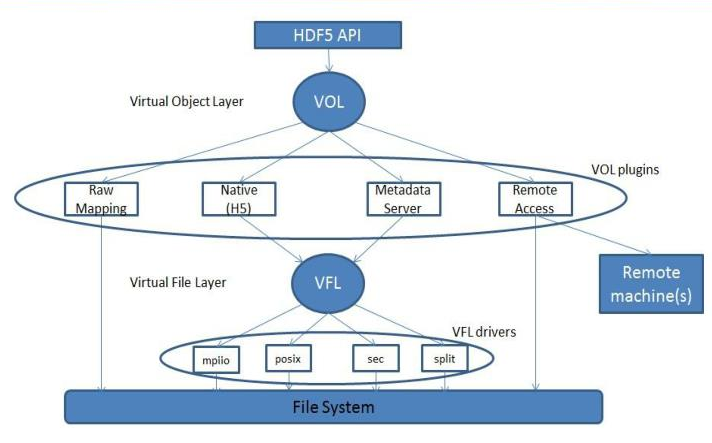
\includegraphics[width=0.9\textwidth]{pictures/vol.png}
		\caption*{VOL Architektur [1]}
	\end{figure}
\end{frame}

%\begin{frame}
	%\frametitle{HDF5 E/A-Problematik}
	%\begin{itemize}
		%\item suboptimale Zugriffsmuster: Simulation vs. Analyse/Verarbeitung
		%\item erfordert häufiges Konvertieren
	%\end{itemize}
%\end{frame}



\section{Projekt: HDF5 Leistungsvergleich}
\begin{frame}
	\frametitle{Projekt: HDF5 Leistungsvergleich}
	\begin{itemize}
		\item Verfügbare HDF5 Implementierungen
			\begin{itemize}
				\item Standard-Implementierung
				\item VOL Implementierung + H5Native-Plugin
			\end{itemize}
	\end{itemize}

	\begin{itemize}
		\item Projektziele
			\begin{itemize}
				\item Leistungs-Messungen
				\item Leistungs-Vergleich
				\item Auswertungsworkflows/-tools
			\end{itemize}
	\end{itemize}
\end{frame}



\section{Projekt: HDF5 shared-memory VOL Plugin}
\begin{frame}
	\frametitle{Projekt: HDF5 shared-memory VOL Plugin}
	%\begin{itemize}
		%\item Sharem Memory (SHMEM)
			%\begin{itemize}
				%\item Dateisystem im Arbeitsspeicher
			%\end{itemize}
	%\end{itemize}

	\begin{itemize}
		\item Projektziele
		\begin{itemize}
			\item Entwicklung eines einfachen Testszenarios
			\begin{itemize}
				\item Kein paralleler Zugriff
				\item Zugriff nur auf eine Datei
			\end{itemize}
			\item Entwicklung der effizienten HDF5-Datenstrukturen
			\item Anpassung von HDF5
			\begin{itemize}
				\item Implementierung eines VOL Plugins
				\item Speichern der HDF5-Daten direkt im Arbeitsspeicher
			\end{itemize}
			\item Benchmarks und Leistungsvergleich zum Native-Plugin
		\end{itemize}
	\end{itemize}
\end{frame}



\section{SIOX Überblick}

\begin{frame}
	\frametitle{SIOX - Scalable E/A for Extreme Performance}
	%\frametitle{\includegraphics[width=0.2\textwidth]{pictures/SIOX_Logo_web_0.png}}
	\begin{itemize}
		\item Leistungsanalyse Analyse Framework
		\item Open-Source-Framework veröffentlich unter LGPL
		\item Unterstützung von diversen E/A-Schichten
			\begin{itemize}
				\item momentan: MPI, POSIX, HDF5 und NETCDF4
			\end{itemize}
		\item Modulares Design
		\item Online-Analyse-Unterstützung
			\begin{itemize}
				\item Aktivitätsanalyse während der Programmausführung
			\end{itemize}
		\item Offline-Analysis-Unterstützung
			\begin{itemize}
				\item Aktivitätsanalyse nach der Programmausführung
			\end{itemize}
	\end{itemize}
\end{frame}

\begin{frame}
	\frametitle{Live-Demonstration}
	\begin{itemize}
		\item Instrumentierung
			\begin{enumerate}
				\item E/A Zugriffe werden erfasst
				\item E/A Zugriffe werden in (SIOX-)Aktivitäten umgewandelt
				\item Aktivitäten werden in einer Datei gespeichert
			\end{enumerate}
		\item PrintPlugin
			\begin{enumerate}
				\item Aktivitäten werden aus der Datei gelesen
				\item Aktivitäten werden im stdout ausgebeben
			\end{enumerate}
		\item FileSurveyor
			\begin{enumerate}
				\item Aktivitäten werden aus der Datei gelesen
				\item Aktivitäten analysiert
				\item Ein Report wird im stdout ausgegeben
			\end{enumerate}
	\end{itemize}
\end{frame}

\section{Projekt: SIOX Analyse-Plugin}
\begin{frame}
	\frametitle{Projekt: SIOX Analyse-Plugin}
	\begin{itemize}
		\item Projektziele
			\begin{itemize}
				\item SIOX Analyse-Plugin
					\begin{itemize}
						\item Aggregation der Informationen
						\item Visualisierung der Zugriffe
						\item Implementierung der verschiedene Sichten
					\end{itemize}
				\item Dokumentation
			\end{itemize}
	\end{itemize}
	\centering
	\begin{figure}
		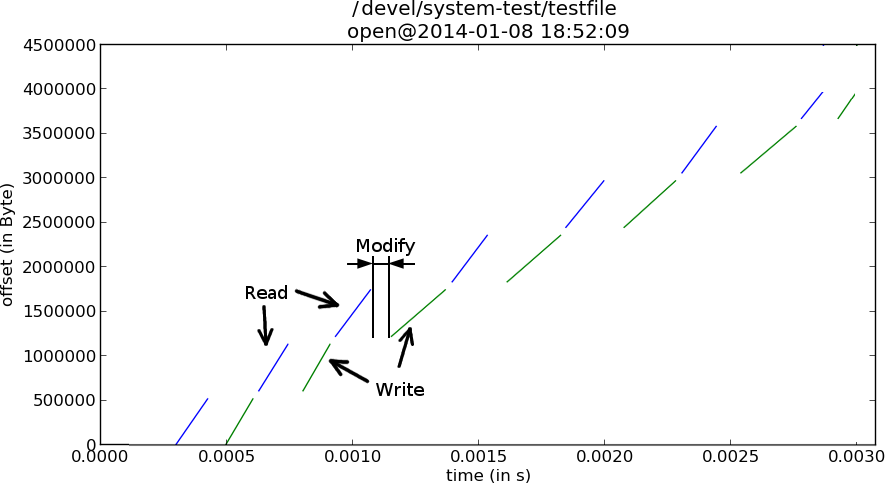
\includegraphics[width=0.6\textwidth]{pictures/p1.png}
		\caption*{Beispiel: AccessInfoPlotterPlugin}
	\end{figure}
\end{frame}

\begin{frame}
	\frametitle{Referenzen}
	\begin{scriptsize}
[1] https://www.hdfgroup.org/why\_hdf

[2] http://www.slideserve.com/gary/virtual-object-layer-in-hdf5
	\end{scriptsize}
\end{frame}

